\section{Performance evaluation}
\label{sec:dssmr-experiments}

In this section, we present the results found for \dssmrappname\ with different
loads and partitionings and compare them with the original
\ssmr{}~\cite{bezerra2014ssmr}. In these experiments, we are interested in
assessing \dssmr{}'s performance with workloads that present different levels of
locality. By locality, we mean the likelihood that certain groups of data items
are accessed together (by the same command). In
Section~\ref{sec:dssmr-evaluation:setup}, we describe the environment where we
conducted our experiments. In Section~\ref{sec:dssmr-evaluation:strongloc}, we
show the results with strong-locality workloads.
In Section~\ref{sec:dssmr-evaluation:weakloc}, we show the results for
weak-locality workloads.

\begin{figure*}
\begin{minipage}[b]{1\linewidth}
\centering
      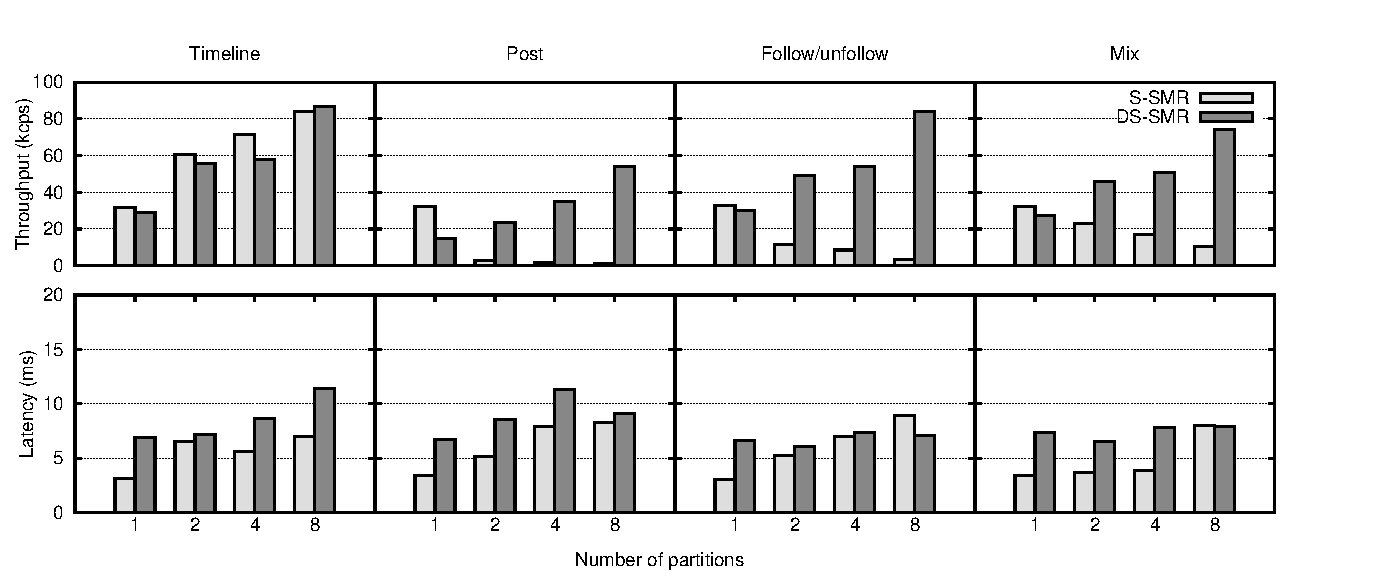
\includegraphics[width=1.08\linewidth]{figures/experiments/dssmr/strong-locality}
\end{minipage}
\caption{Results of \dssmrappname\ running with \ssmr\ and \dssmr{} with strong-locality workload. Throughput is shown in thousands of commands per second (kcps).}
\label{fig:dssmr-strongloc}
\end{figure*}

\subsection{Environment setup and configuration parameters}
\label{sec:dssmr-evaluation:setup}

We conducted all experiments on a cluster that had two types of nodes: (a) HP
SE1102 nodes, equipped with two Intel Xeon L5420 processors running at 2.5 GHz
and with 8 GB of main memory, and (b) Dell SC1435 nodes, equipped with two AMD
Opteron 2212 processors running at 2.0 GHz and with 4 GB of main memory. The HP
nodes were connected to an HP ProCurve 2920-48G gigabit network switch, and the
Dell nodes were connected to another, identical switch. Those switches were
interconnected by a 20 Gbps link. All nodes ran CentOS Linux 7.1 with kernel
3.10 and had the OpenJDK Runtime Environment~8 with the \mbox{64-Bit} Server VM
(build 25.45-b02).
%We kept the clocks synchronized using NTP in order to measure latency
%components involving events in different computers.

For the experiments, we use the following workloads: Timeline (composed only of
getTimeline requests), Post (only post requests), Follow/unfollow (50\% of
follow requests and 50\% of unfollow), and Mix (7.5\% post, 3.75\% follow,
3.75\% unfollow, and 85\% getTimeline).

\subsection{Results for strong locality}
\label{sec:dssmr-evaluation:strongloc}

% THROUGHPUT

We can see in Figure~\ref{fig:dssmr-strongloc} and Table~\ref{tbl:results} the
results achieved with \dssmrappname{}, running with a strong-locality workload.
For the Timeline workload, the throughput with \dssmr\ and \ssmr\ are very
similar. This happens because getTimeline requests are optimized to be
single-partition: all posts in a user's timeline are stored along with the User
object. Every getTimeline requests accesses a single User object (of the user
whose timeline is being requested). This is the ideal workload for \ssmr{}. In
\dssmr{}, the partitioning does not change, and consulting the oracle becomes
unnecessary thanks to the local cache at each client. This happens because there
are no other commands in the Timeline workload.

In the Post workload, every command accesses up to all partitions in the system,
which is the worst case for \ssmr{}: the more partitions are involved in the
execution of a command, the worst is the system's performance. We can see that
the throughput of \ssmr\ decreases significantly as the number of partitions
increases. For \dssmr{}, we can see that the system throughput scales with the
number of partitions. This happens because User objects that are accessed
together, but which are in different partitions, are moved to the same partition
based on the interests of the users. As the execution proceeds, this leads to a
lower rate of multi-partition commands, which allows throughput to scale. (In
the case of posts on 2 partitions, the number of move commands started at 3
kcps, with throughput of 23 kps, and eventually reduced to less than 0.1 kcps.)
As a result the throughput improvement of \dssmr{} with respect to \ssmr\
increases over time. With eight partitions, \dssmr{} sports a performance that
is 45 times that of \ssmr!

With the Follow/unfollow workload, the system performs in a similar way to that
observed with the Post workload. The difference is that each follow or unfollow
request accesses only two User objects, whereas every post request may affect an
unbounded number of users. For this reason, each follow/unfollow command is
executed at most by two partitions in \ssmr{}. In \dssmr{}, a single move
command is enough to have all User objects affected by such a command in the
same partition. For this reason, both replication techniques have better
throughput under the Follow/unfollow workload than with Post. As with the Post
workload, \dssmr{}'s advantage over \ssmr\ increases with the number of
partitions, reaching up to almost 25 times with eight partitions.

We approximate a realistic distribution of commands with the Mix workload. With
such a workload, \ssmr\ does not perform as bad as in the Post or
Follow/unfollow workloads, but the system throughput still decreases as
partitions are added. As with the other workloads, \dssmr\ scaled under the Mix
workload. With eight partitions, it reached 74~kcps (thousands of commands per
second), fairly close to the ideal case (the Timeline workload), where \dssmr\
reached 86~kcps. Under the Mix workload, \ssmr\ had less than 33~kcps in the
best case (one partition) and around 10~kcps with eight partitions. In the
configuration with eight partitions, \dssmr\ reaches almost seven times \ssmr's
throughput.

Latency values with \dssmr\ are higher than with \ssmr{}. This was expected for
two reasons. First, there is an extra group of servers (the oracle) to
communicate with. Second, executing a command often means moving all accessed
objects to the same partition. Taking this into account, we consider the (often
slight) increase in latency observed with \dssmr\ a low price to pay for the
significant increase in throughput and the scalability that \dssmr\ brought to
the system; with \ssmr{}, the system did not scale with multi-partition
commands.

\begin{table*}[htp]
      \vspace{10mm}
      \caption{Absolute values of \dssmrappname\ running \ssmr\ and \dssmr{}.}
      \centering
      \begin{adjustbox}{max width=\textwidth}
      \begin{tabular}{|l|c|c|c|c|c|c|c|c|c|c|c|c|c|c|c|c|} \hline
               & \multicolumn{4}{|c|}{Timeline}  &  \multicolumn{4}{|c|}{Post}   &  \multicolumn{4}{|c|}{Follow/unfollow}  &  \multicolumn{4}{|c|}{Mix}    \\ \hline
               & 1     & 2     & 4     & 8       & 1     & 2     & 4   & 8    & 1     & 2     & 4       & 8           & 1     & 2     & 4     & 8     \\ \hline\hline
               & \multicolumn{16}{|c|}{Throughput (commands per second)} \\ \hline
      \ssmr\   & 31757 & 60699 & 71274 & 84065   & 32151 & 2884  & 1894  & 1200  & 32541 & 11476 & 8580    & 3371          & 32151 & 22803 & 16822 & 10657 \\ \hline
      \dssmr\  & 28882 & 55925 & 57900 & 86685   & 14874 & 23295 & 35188 & 54250 & 30215 & 48976 & 54025   & 83880         & 27101 & 45686 & 50671 & 74257 \\ \hline\hline
               & \multicolumn{16}{|c|}{\textbf{Throughput rate = \dssmr\ tput / \ssmr\ tput}} \\ \hline
               & \textbf{0.91} & \textbf{0.92}  & \textbf{0.81} & \textbf{1.03}     & \textbf{0.46}   & \textbf{8.08}   & \textbf{18.48}  & \textbf{45.00} & \textbf{0.93} & \textbf{4.27} & \textbf{6.30} & \textbf{24.88} & \textbf{0.84} & \textbf{2.00} & \textbf{3.01} & \textbf{6.97} \\ \hline\hline
               & \multicolumn{16}{|c|}{Latency (milliseconds)} \\ \hline
      \ssmr\   & 3.1 & 6.6 & 5.6 & 7.0  & 3.4 & 5.2  & 7.9  & 8.3  & 3.0  & 5.2  & 7.0  & 8.8  & 3.4  & 3.7  & 3.8  & 7.9  \\ \hline
      \dssmr\  & 6.9 & 7.1 & 8.6 & 11.4 & 6.7 & 8.6  & 11.3 & 9.1  & 6.6  & 6.1  & 7.4  & 7.0  & 7.3  & 6.5  & 7.8  & 7.9  \\ \hline
      \end{tabular}
      \end{adjustbox}
      \label{tbl:results}
      \vspace{10mm}
\end{table*}%


\subsection{Results for weak locality} \label{sec:dssmr-evaluation:weakloc}

\begin{figure*}
\begin{minipage}[b]{1\linewidth}
\centering
      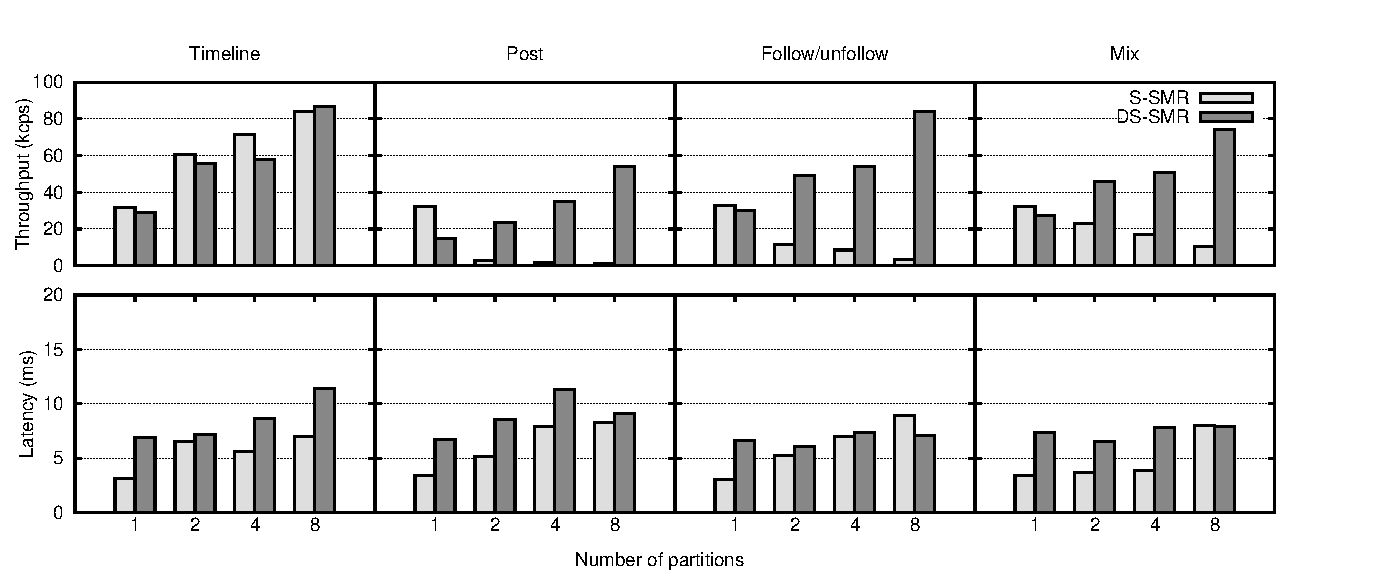
\includegraphics[width=1.08\linewidth]{figures/experiments/dssmr/weak-locality}
\end{minipage}
\caption{Results of \dssmrappname\ running with \ssmr\ and \dssmr{} with weak-locality workload. Throughput is shown in thousands of commands per second (kcps).}
\label{fig:dssmr-weakloc}
\end{figure*}

The Figure~\ref{fig:dssmr-weakloc} shows the results achieved with
\dssmrappname{}, running with a weak-locality workload.

\fxnote{Add few more words on this performance. [Should we include this here?]}
